\documentclass[12pt, a4paper]{article}
\usepackage{titlesec}
\usepackage{graphicx}
\usepackage{amsmath}
\renewcommand{\figurename}{Att.}
\titlelabel{\thetitle.\quad}
\author{Pēteris Račinskis pr20015}
\date{19/12/21}
\begin{document}
\title{5. mājas darbs}

\maketitle

\section{Uzdevums}

Definējot grafa sakarības skaitli $k(G)$ kā minimālo nešķeļošu virsotņu ceļu skaitu starp katru grafa virsotņu pāri, nesakarīgam grafam $k(G)=0$, pilnam grafam - $k(G)=n-1$
Attiecīgi sekojošā konstrukcija izpilda uzdevuma nosacījumus.

\begin{figure}[h!]
    \centering
    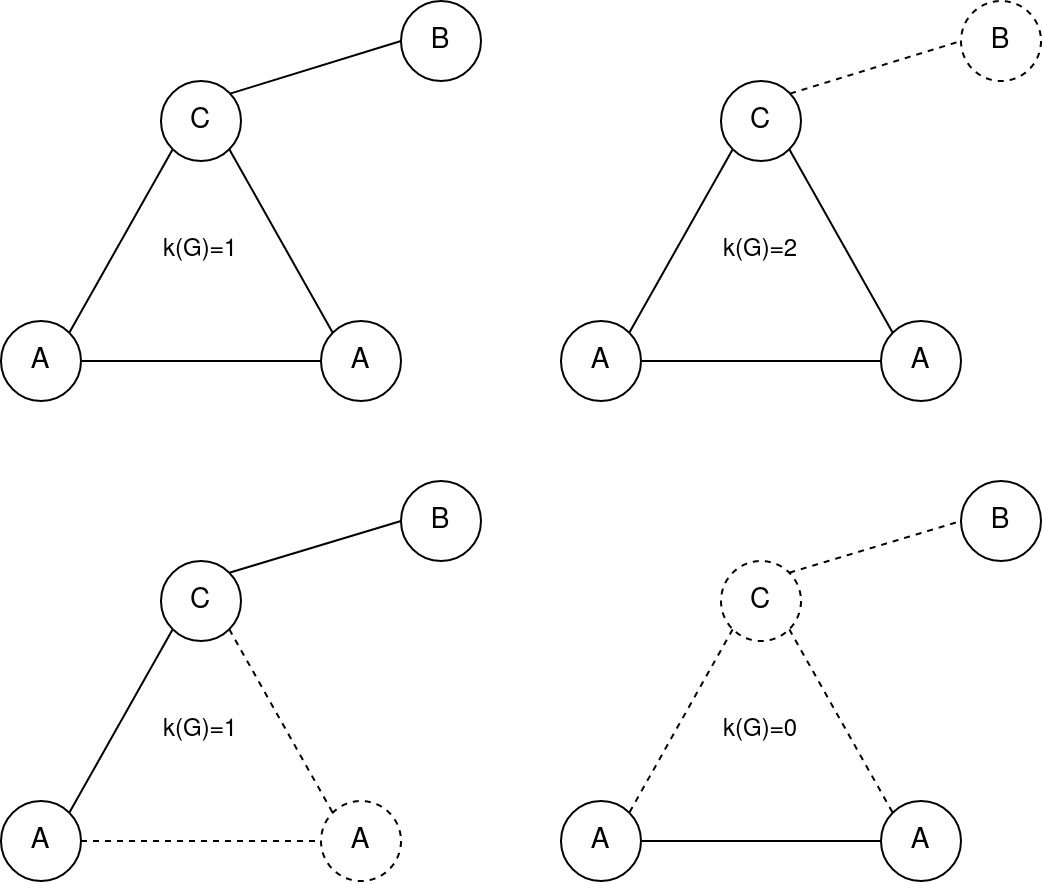
\includegraphics[height=10cm,page=1]{task-1.jpeg}
    \caption{Grafa sakarības skaitļa izmaiņas, izmetot virsotnes.}
\end{figure}

\newpage
\section{Uzdevums}

Jebkurš Petersena grafa apakšgrafs, kas iegūts, izmetot vienu virsotni, nav planārs, jo ir reducējams uz $K_{3,3}$, veicot šķautņu savilkšanas visām palikušajām virsotnēm ar $deg=2$:

\begin{figure}[h!]
    \centering
    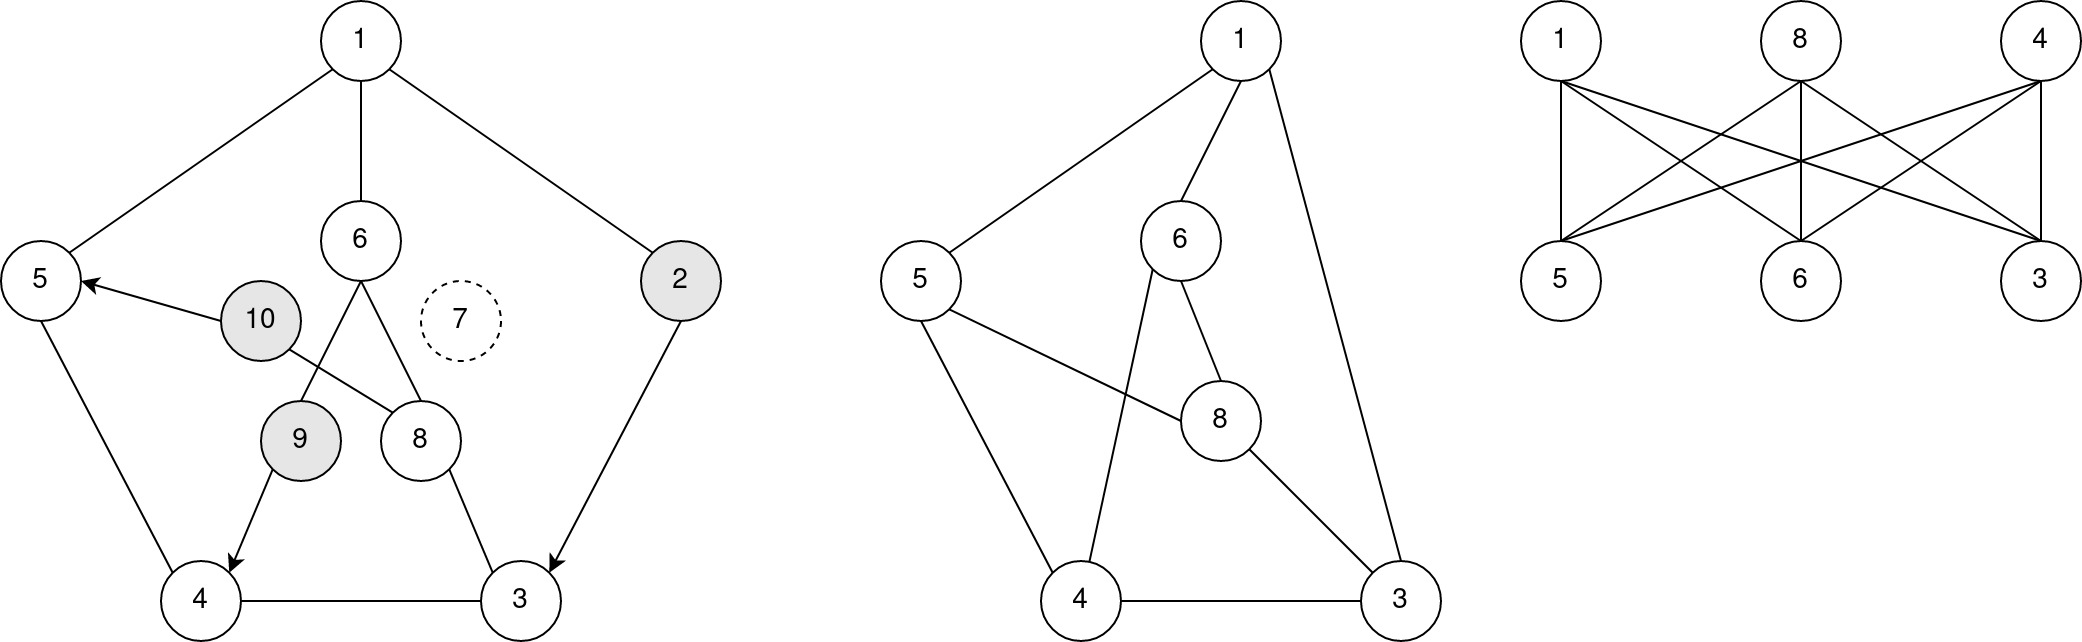
\includegraphics[height=4cm,page=1]{task2-1.jpeg}
\end{figure}

Petersena grafa apakšgrafs, kas iegūts, divām blakus esošām virsotnēm atmetot citu šķautni, ir planārs:

\begin{figure}[h!]
    \centering
    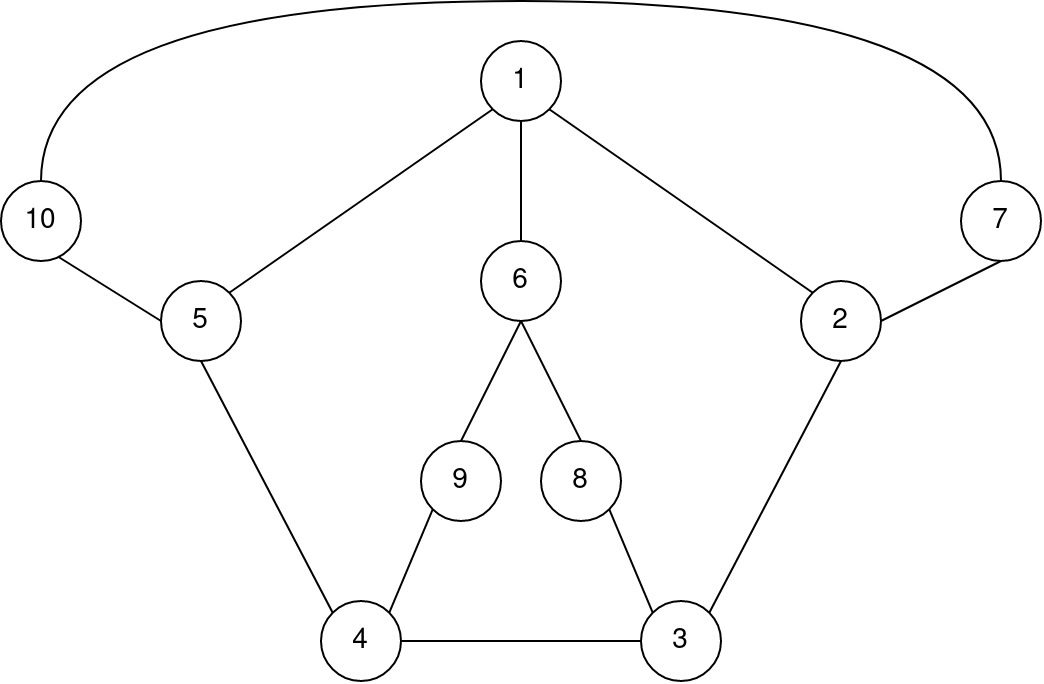
\includegraphics[height=4cm,page=1]{task2-2.jpeg}
\end{figure}

Pievienojot atpakaļ jebkuru no šķautnēm (10-8 vai 7-9) attēlā, iespējams atkārtot augstāk attēloto redukciju uz $K_{3,3}$, tāpēc katra no šķautnēm noteikti šķērsos vismaz vienu citu jau pastāvošo. Līdz ar to Petersena grafs ar minimālu krustojumu skaitu ir ar diviem krustojumiem:

\begin{figure}[h!]
    \centering
    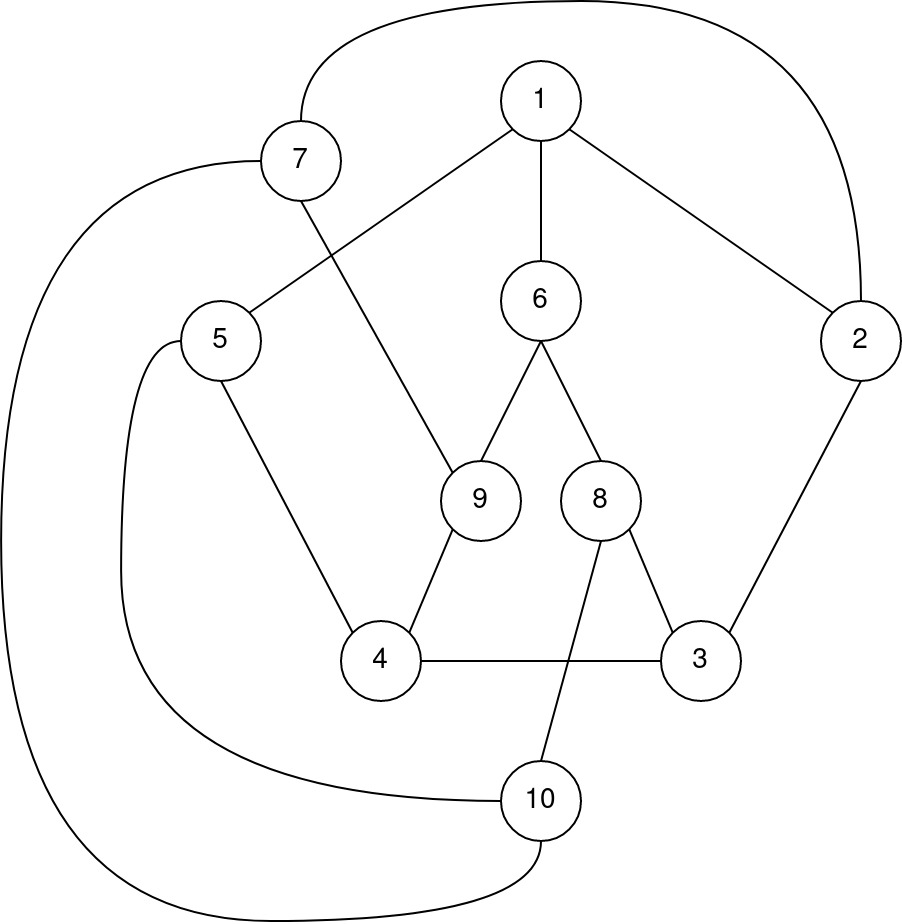
\includegraphics[height=4cm,page=1]{task2-3.jpeg}
\end{figure}


\newpage
\section{Uzdevums}

Hamiltona cikla pastāvēšanas nosacījums 3-regulārā grafā: pastāv krāsojums 3 krāsās. k-regulārā grafā ekvivalenta problēma ir 1-faktorizācija (redukcija uz 1-regulāriem apakšgrafiem ar to pašu virsotņu kopu - 1-faktoriem - kuru šķautņu kopas ir nešķeļošas). Tāpat ir jābūt arī pilnajam sapārojamam (1-faktoram), kas nešķeļ Hamiltona ceļu.

Petersena grafā veidojot 1-faktoru (pilnā sapārojumu) nešķeļošu apakš-grafu, sākot ar jebkuru šķautni, un pa vienai izmetot palikušās šķautnes tā, lai palikušajā grafā visām virsotnēm $deg=2$, var pierādīt, ka iespējami tikai divi varianti (konstrukcija ir vienāda visām virsotņu secībām). Abos gadījumos pārējās šķautnes veido divus 5-ciklus, nevis vienu Hamiltona ciklu. Šādas 5-cikla komponentes arī nav iespējams 1-faktorizēt (nokrāsot divās palikušajās krāsās), jo jebkurā gadījumā vienai virsotnei ciklā paliks $deg=2$ vai $deg=0$ (abas šķautnes būs vienā krāsā).

\begin{figure}[h!]
    \centering
    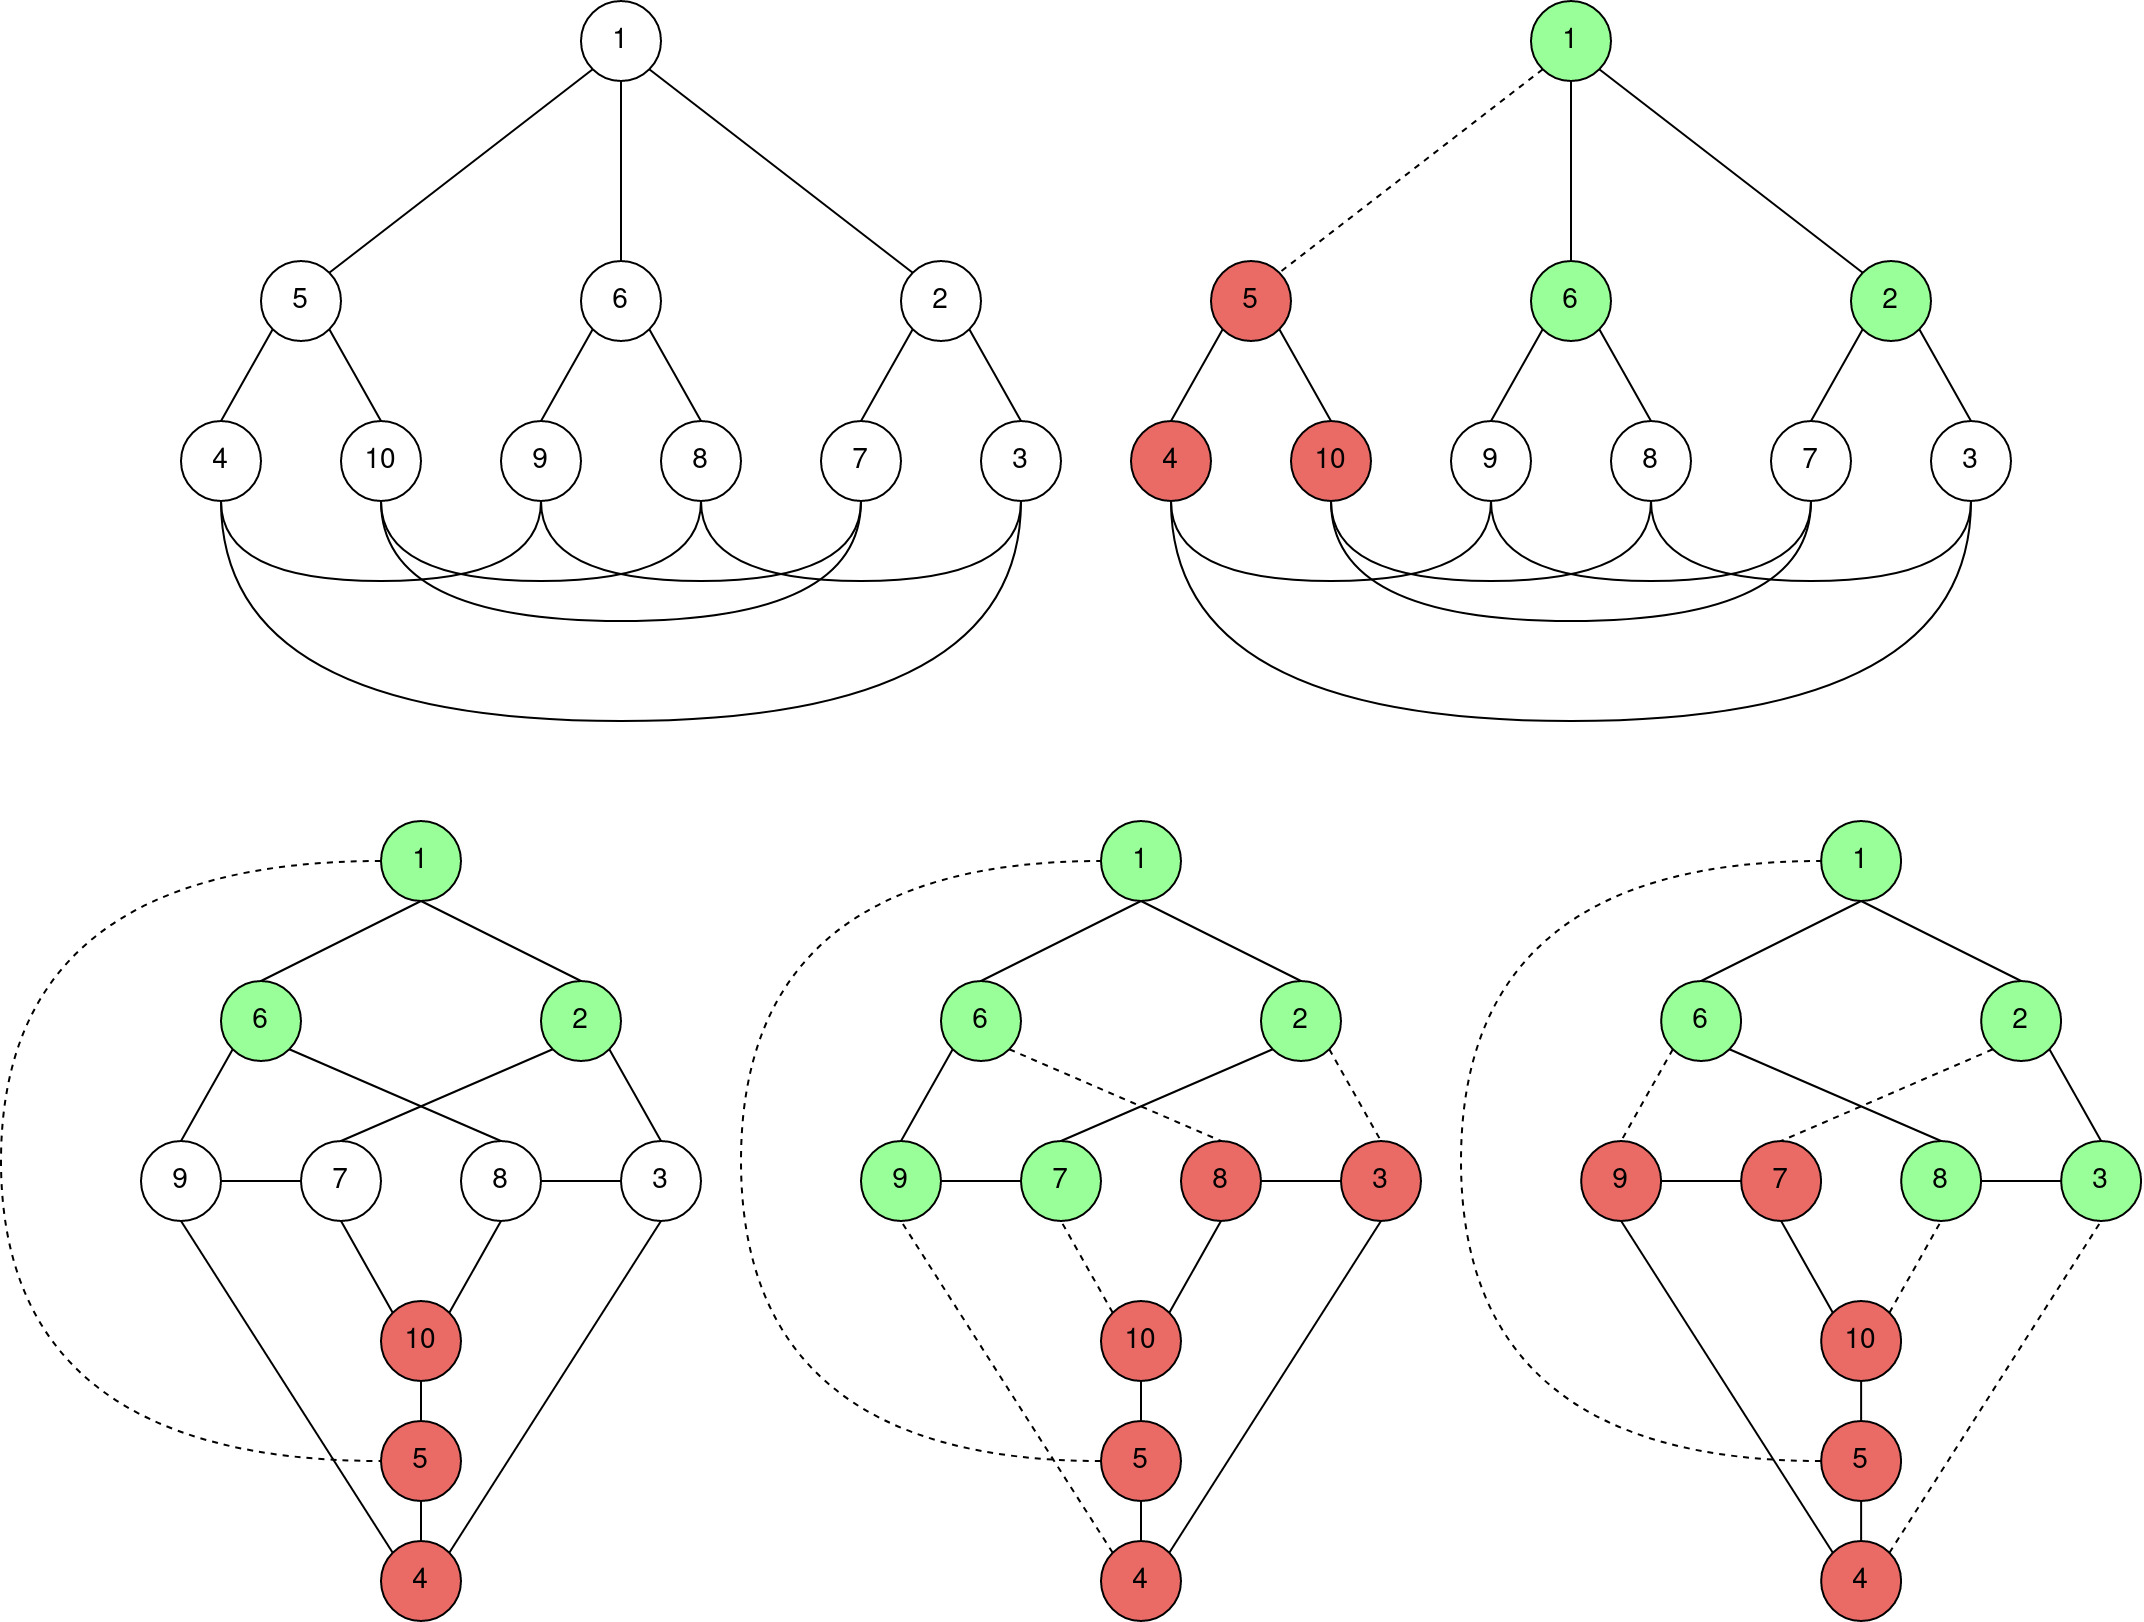
\includegraphics[height=8.9cm,page=1]{task3.jpeg}
\end{figure}
Sākot ar jebkuru šķautni, ir iespējami tikai divi pilnie sapārojumi kā palikušo grafu nešķeļoši sākotnējā grafa faktori. Izmetot šķautni, katru tās virsotni un visas tai blakus esošās virsotnes palikušajā grafā marķē kādā krāsā. Šķautni nevar izmest no grafa, ja abas tās virsotnes ir marķētas vienā krāsā, jo katrai virsotnei rezultātā jābūt $deg=2$. Mēģinot citādi dalīt grafu otrajā attēla rindā, tiek iegūta situācija, kad vai nu jāatstāj virsotnes ar $deg=3$, vai arī jāizmet šķautnes līdz kādai ir $deg=1$.

\end{document}